%=======================+=========================
%==============  Trigger    ================
%=================================================\

\section{Trigger (Sasha) \label{sec:trig}}
\subsection{Architecture \label{sec:trigarchitecture}}
The goal of the GlueX trigger is to accept most high-energy hadronic interactions while reducing the background rate induced by electromagnetic and low-energy hadronic interactions leading to an overall rate of about 80 kHz, which is acceptable by the DAQ.  The trigger system of the GlueX experiment\cite{GlueX:2013twa} is implemented on pipelined special-purpose programmable electronics modules with Field-Programmable Gate Array (FPGA) chips. The modules were designed at Jefferson Lab.  The GlueX trigger and read out electronics is hosted in VXS (ANSI/VITA 41.0) crates; VXS is an extension of the VME/VME64x architecture, that implements high-speed backplane lines used to transmit trigger information. The main trigger algorithm is 
based on measurement of the energy depositions in two electromagnetic calorimeters~\cite{somov_l1}. Supplementary triggers can also
use hits from scintillator detectors, such as the PS, tagging detectors, ST, and TOF.

A layout of the trigger system is presented in Fig.~\ref{fig:trig}. Data from the Forward and Barrel calorimeters are sent to  Flash ADC (FADC250)~\cite{Dong:2007} modules, situated in 12 and 8 VXS crates, respectively, and are digitized at the sampling rate of 250 MHz. The digitized amplitudes are used for the trigger and are also stored in the FADC FPGA-based pipeline for the subsequent readout via VME.
Digitized amplitudes are summed for all 16 FADC250 channels in each 4 ns sampling interval and are transmitted to the crate trigger processor (CTP) module, which sums up amplitudes from all FADC boards in the crate. The sub-system processor (SSP) modules located in the global trigger crate receives amplitudes from all crates and computes the total energy deposited in the FCAL and BCAL. The global trigger processor (GTP) module collects data from the SSPs, performs computation of different trigger equations and makes the trigger decision. The core of the trigger system is the trigger supervisor (TS) module. It receives the trigger information from the GTP and distributes triggers to electronics modules in all readout 
crates in order to initiate the data readout. There are 55 VXS crates in total in GlueX (26 with FADC250s, 14 with  FADC125s, 14 with F1 TDCs, and 1 CAEN TDC). The TS also provides a synchronization of all crates and sends a 250 MHz clock signal. The triggers and clock are distributed through the trigger distribution (TD) module in the trigger distribution crate and the trigger interface (TI) module and signal distribution (SD) module in each readout crate. The GlueX trigger system provides a fixed latency of about 3.1 $\mu$s.

\begin{figure}[tbp]
\begin{center}
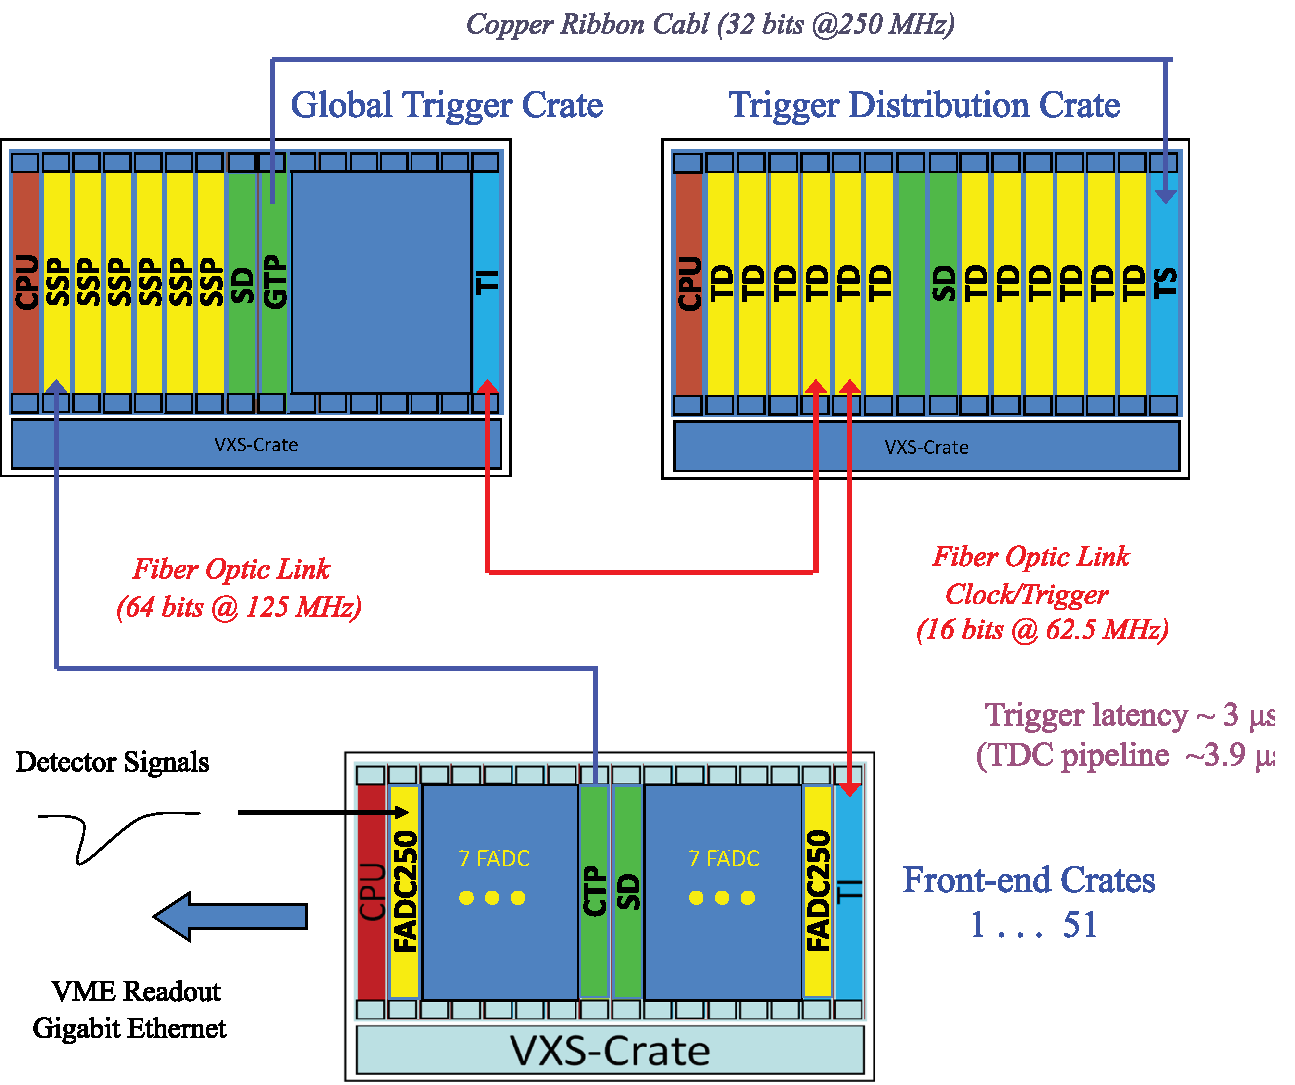
\includegraphics[width=0.75\textwidth]{figures/125_Somov-f1.pdf}  
\caption{Schematic view of the Level-1 trigger system of the GlueX experiment. Description of the electronics boards is given in the text.} \label{fig:trig}
\end{center}
\end{figure}

\subsection{Trigger Types \label{sec:triggers}}

The GlueX experiment uses two main trigger types: the pair spectrometer trigger, and the physics trigger based on energy depositions in the BCAL and FCAL. The 
pair spectrometer trigger is used to measure the flux of beam photons. This trigger requires a time coincidence of hits in the 
two arms of the PS detector, which is described in Section~\ref{sec:ps}. The physics triggers are generated when the FCAL and BCAL energies  satisfy the following equations (1) $2\cdot E_{\rm FCAL} + E_{\rm BCAL} > 1\;{\rm GeV}$,  $E_{\rm FCAL} > 0\; {\rm GeV}$ and (2) $E_{\rm BCAL} > 1.2\;{\rm GeV}$. The latter trigger type is used to accept events with large transverse energy released in the BCAL, such as decays of $J/\psi$ mesons.
Several other trigger types were implemented for efficiency studies and detector calibration. Ancillary minimum-bias random trigger, 
and calorimeter LED triggers were used concurrently with data taking. The rate of the random trigger and each of the LED triggers constituted 100 Hz and 10 Hz, respectively.

\subsection{Performance \label{sec:trigperformance}}
The rate of the main physics triggers as a function of the pair 
spectrometer trigger rate is shown in Fig.~\ref{fig:trig_rate}.
The typical rate of the PS trigger in the spring of 2018 was 3.5 kHz, which corresponds to a photon beam flux of about $2.5\cdot 10^7\; \gamma/{\rm sec}$ in the GlueX energy range of interest. The total trigger rate was about 40 kHz. The electronics and DAQ were running with the live time close to 
$100 \%$, collecting data from the GlueX detector at a rate of 600 megabytes per second.

%In spring 2018, data were collected at the luminosity %corresponding to the photon beam flux of about $2.5\cdot 10^7\; %\gamma/{\rm sec}$ in the GlueX energy range of interest. The %typical rate of the PS trigger 

\begin{figure}[tbp]
\begin{center}
\includegraphics[width=0.75\textwidth]{figures/Rate_diamond_2018.png}  
\caption{Rate of the main production triggers as a function of the PS rate: FCAL \& BCAL trigger (boxes), BCAL trigger (triangles), the total trigger rate (circles). The vertical arrow indicates the run condition corresponding to the spring run of 2018.} \label{fig:trig_rate}
\end{center}
\end{figure}
